\documentclass[14pt]{extarticle}
\usepackage[paperwidth=16cm,paperheight=9cm,margin=0.8cm]{geometry}
\usepackage{graphicx,booktabs,xcolor}
\usepackage[hidelinks]{hyperref}
\pagestyle{empty}
\definecolor{navy}{HTML}{142638}
\definecolor{teal}{HTML}{08796C}
\setlength{\parindent}{0pt}
\newcommand{\heading}[1]{{\color{teal}\small UCS503P / REVIVE}\par\medskip{\color{navy}\LARGE\bfseries #1}\par\medskip}
\begin{document}
\renewcommand{\labelitemi}{\(\bullet\)}
\heading{ReVive}
\Large Explainable financial anomaly detection\par
\medskip\normalsize Final Software Engineering seminar\par
\vfill Aakriti Sharma, Koena, Mayur Goyal\par TIET Patiala
\newpage
\heading{What reviewers need}
A ranked set of suspicious transaction windows and enough evidence to investigate each flag.
\begin{itemize}
\item Upload public transaction data or run a synthetic example.
\item Inspect the anomaly timeline and explanations.
\item Review the triage tier and stored alert history.
\end{itemize}
\newpage
\heading{System architecture}
\begin{center}
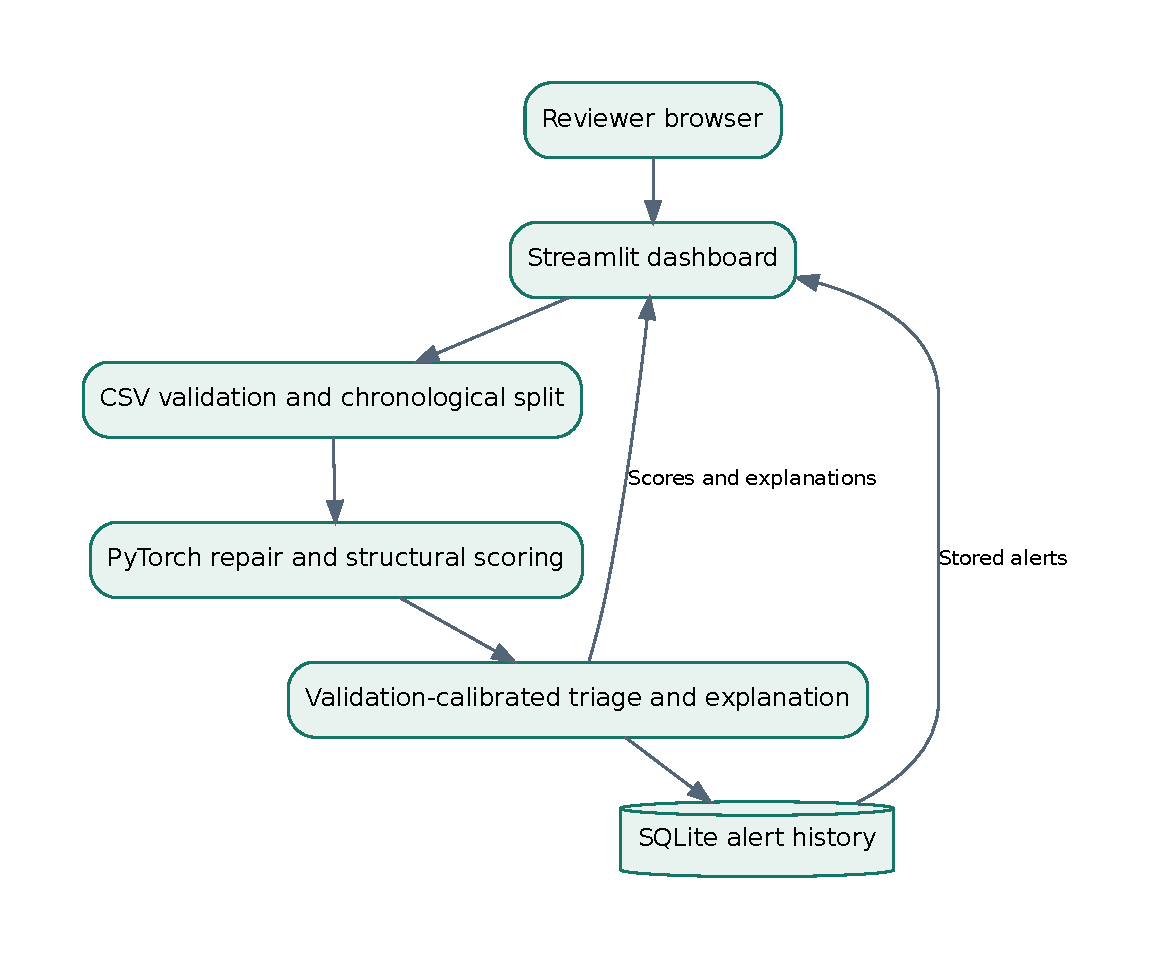
\includegraphics[height=4.6cm]{architecture.pdf}
\end{center}
\newpage
\heading{Held-out benchmark}
First 8,000 ULB transactions. Chronological split, 50-row windows, stride 5, seed 42.
\medskip

\begin{tabular}{lrr}
\toprule Detector & Avg. precision & ROC-AUC\\
\midrule ReVive & 0.9681 & 0.9894\\
Isolation Forest & 0.3249 & 0.6646\\
Local Outlier Factor & 0.4914 & 0.8161\\
\bottomrule
\end{tabular}
\newpage
\heading{Calibration cut review workload}
\begin{tabular}{lrrr}
\toprule Policy & Flagged & Precision & Recall\\
\midrule Original defaults & 626 & 21.57\% & 100\%\\
Validation calibrated & 338 & 39.94\% & 100\%\\
\bottomrule
\end{tabular}
\medskip

Both policies used the same 631 test windows. Calibration retained all 135 positive windows in this subset. The remaining alert rate was 53.57\%.
\newpage
\heading{Verification and live demo}
\begin{itemize}
\item Checked valid and invalid CSV input, triage, and explanation output.
\item Reopened the app and recovered 338 alerts from the local SQLite file.
\item Repeated the seeded experiment and reproduced both displayed tables.
\end{itemize}
\href{https://revive2627.streamlit.app/}{\textcolor{teal}{Open the live dashboard}}
\newpage
\heading{Limits and next steps}
The recorded result covers overlapping windows in one chronological subset. Anonymized features limit business interpretation, and hosted SQLite can reset.
\medskip

Next steps are to evaluate additional holdouts and tune thresholds against a reviewer capacity target.
\newpage
\heading{Class diagram}
\begin{center}
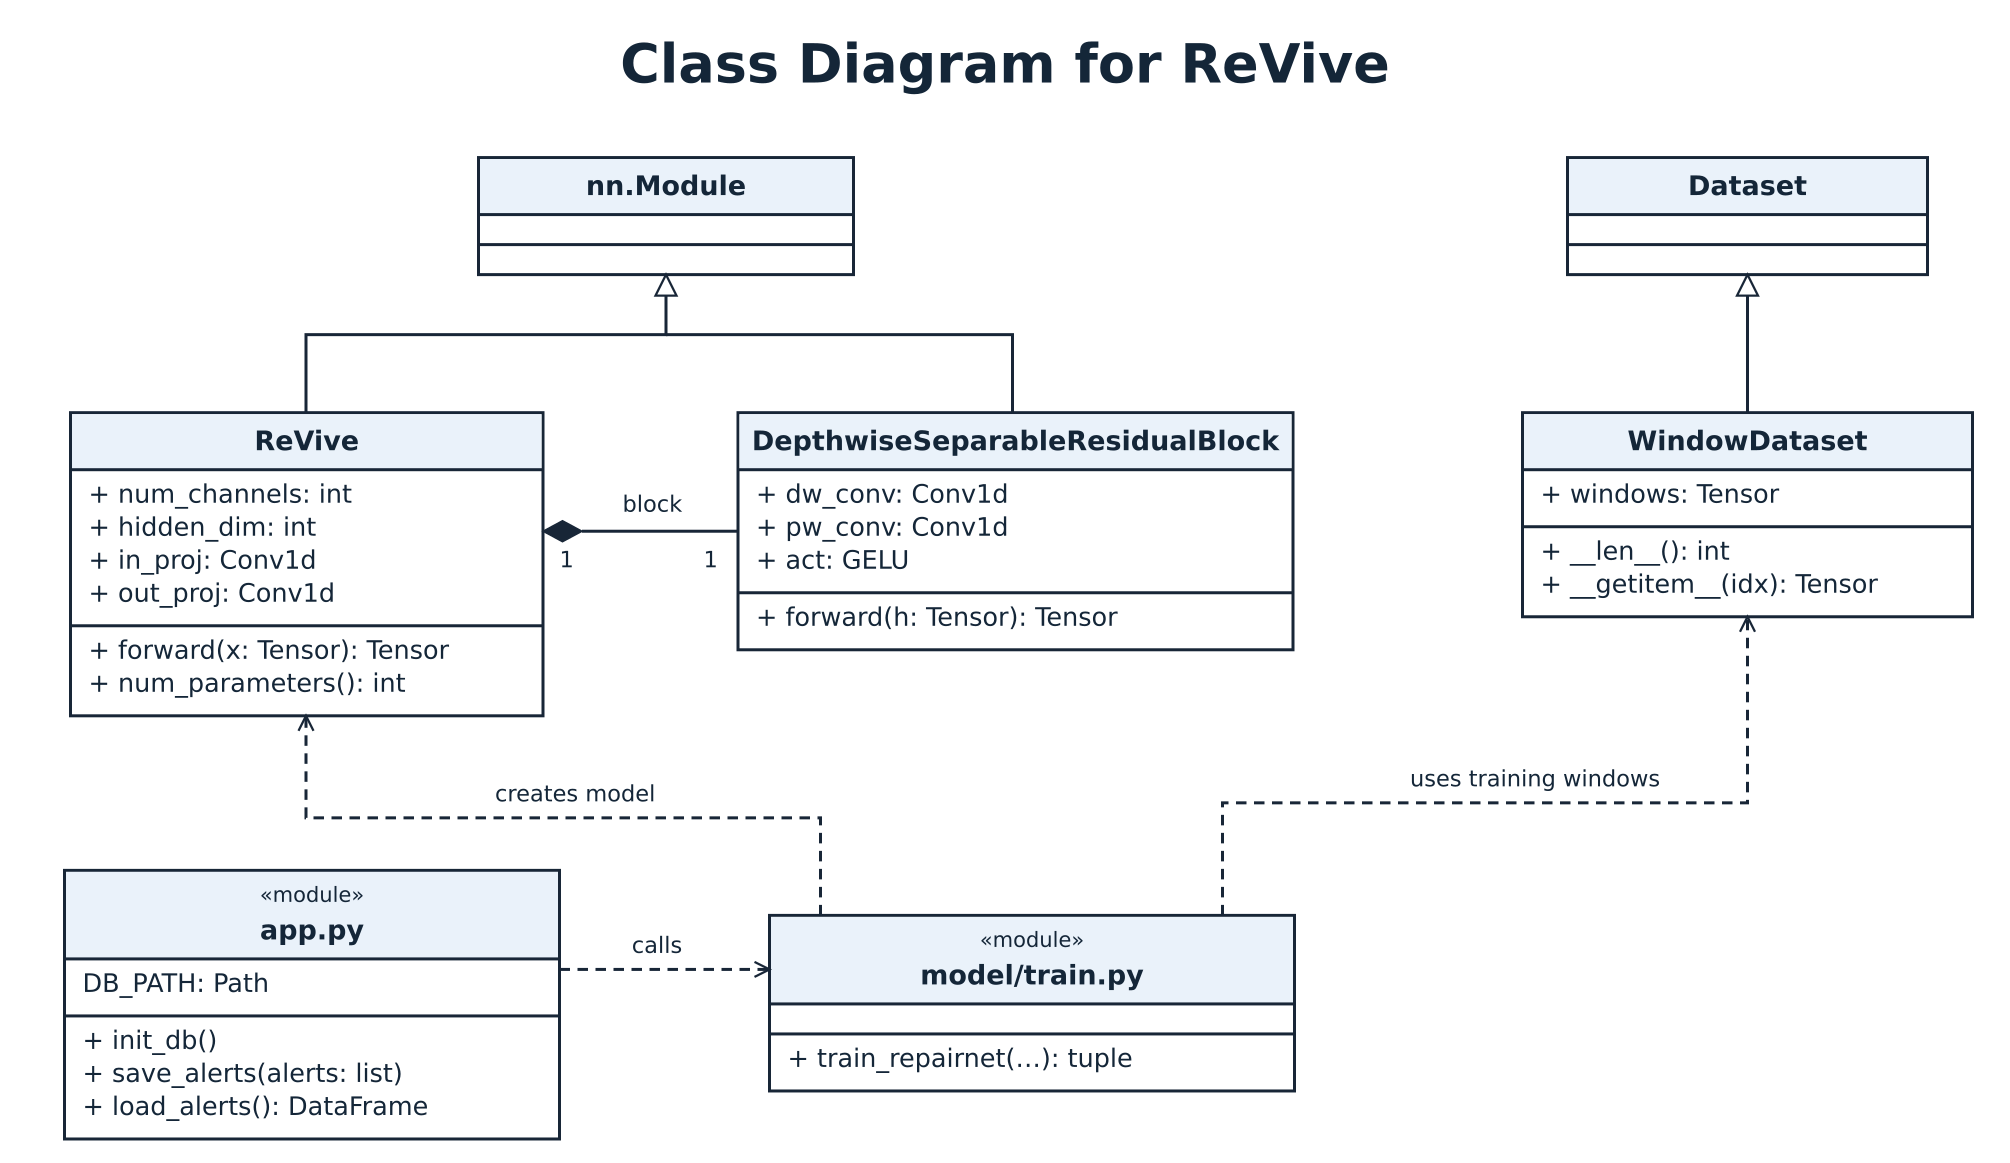
\includegraphics[width=\linewidth,height=4.65cm,keepaspectratio]{../docs/images/class-diagram.png}
\end{center}
\newpage
\heading{Level 0 data flow diagram}
\begin{center}
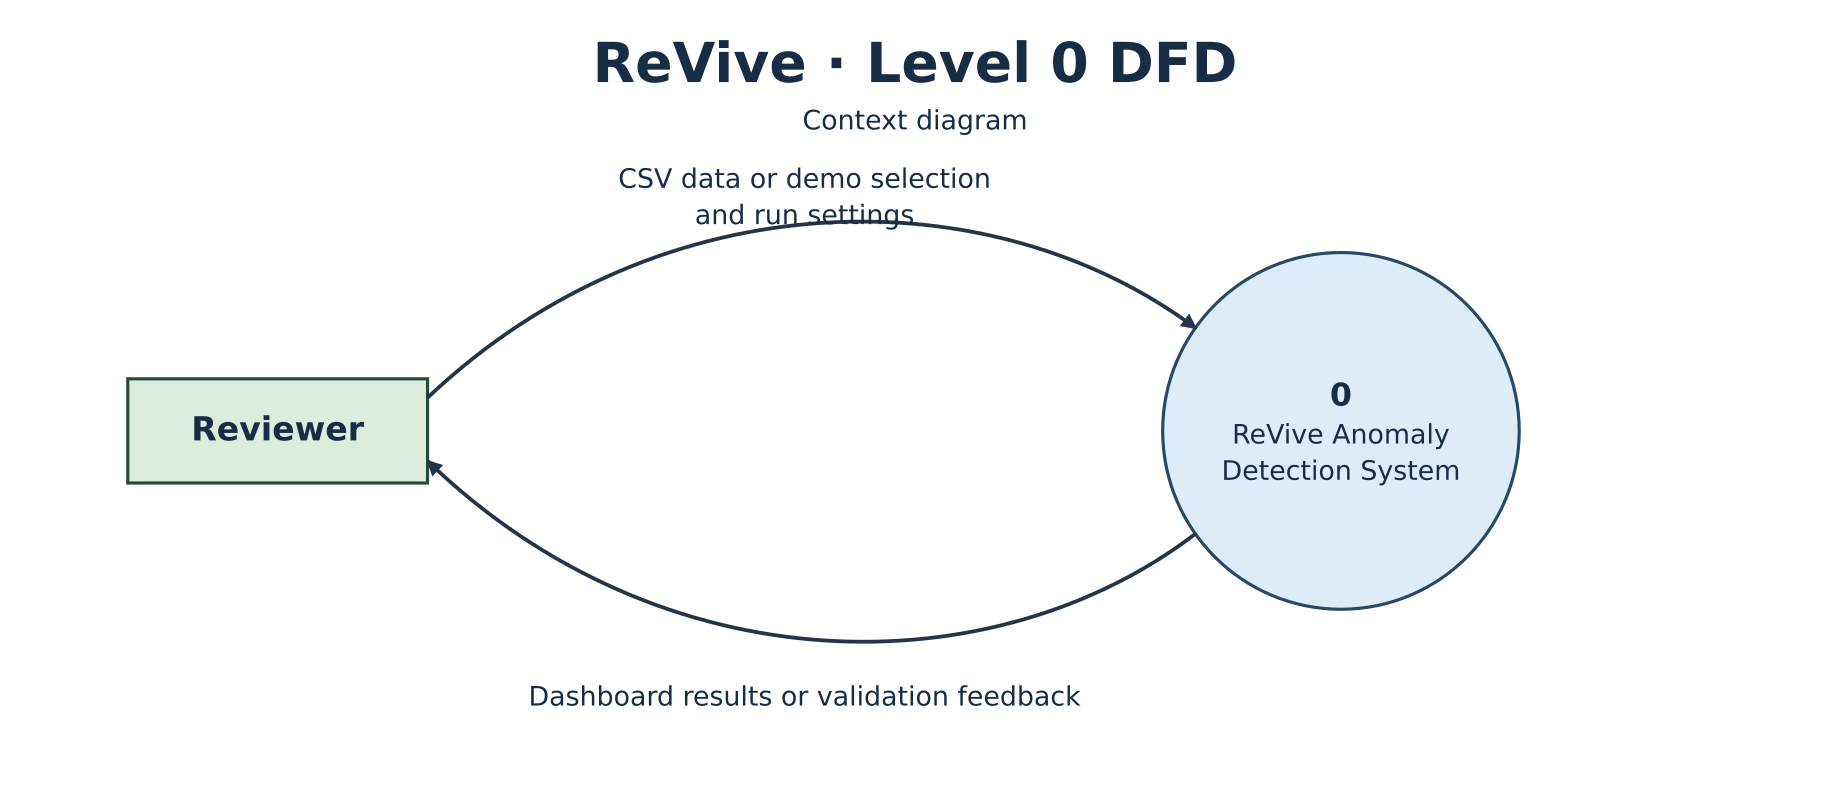
\includegraphics[width=\linewidth,height=4.65cm,keepaspectratio]{../docs/images/dfd-level-0.png}
\end{center}
\newpage
\heading{Level 1 data flow diagram}
\begin{center}
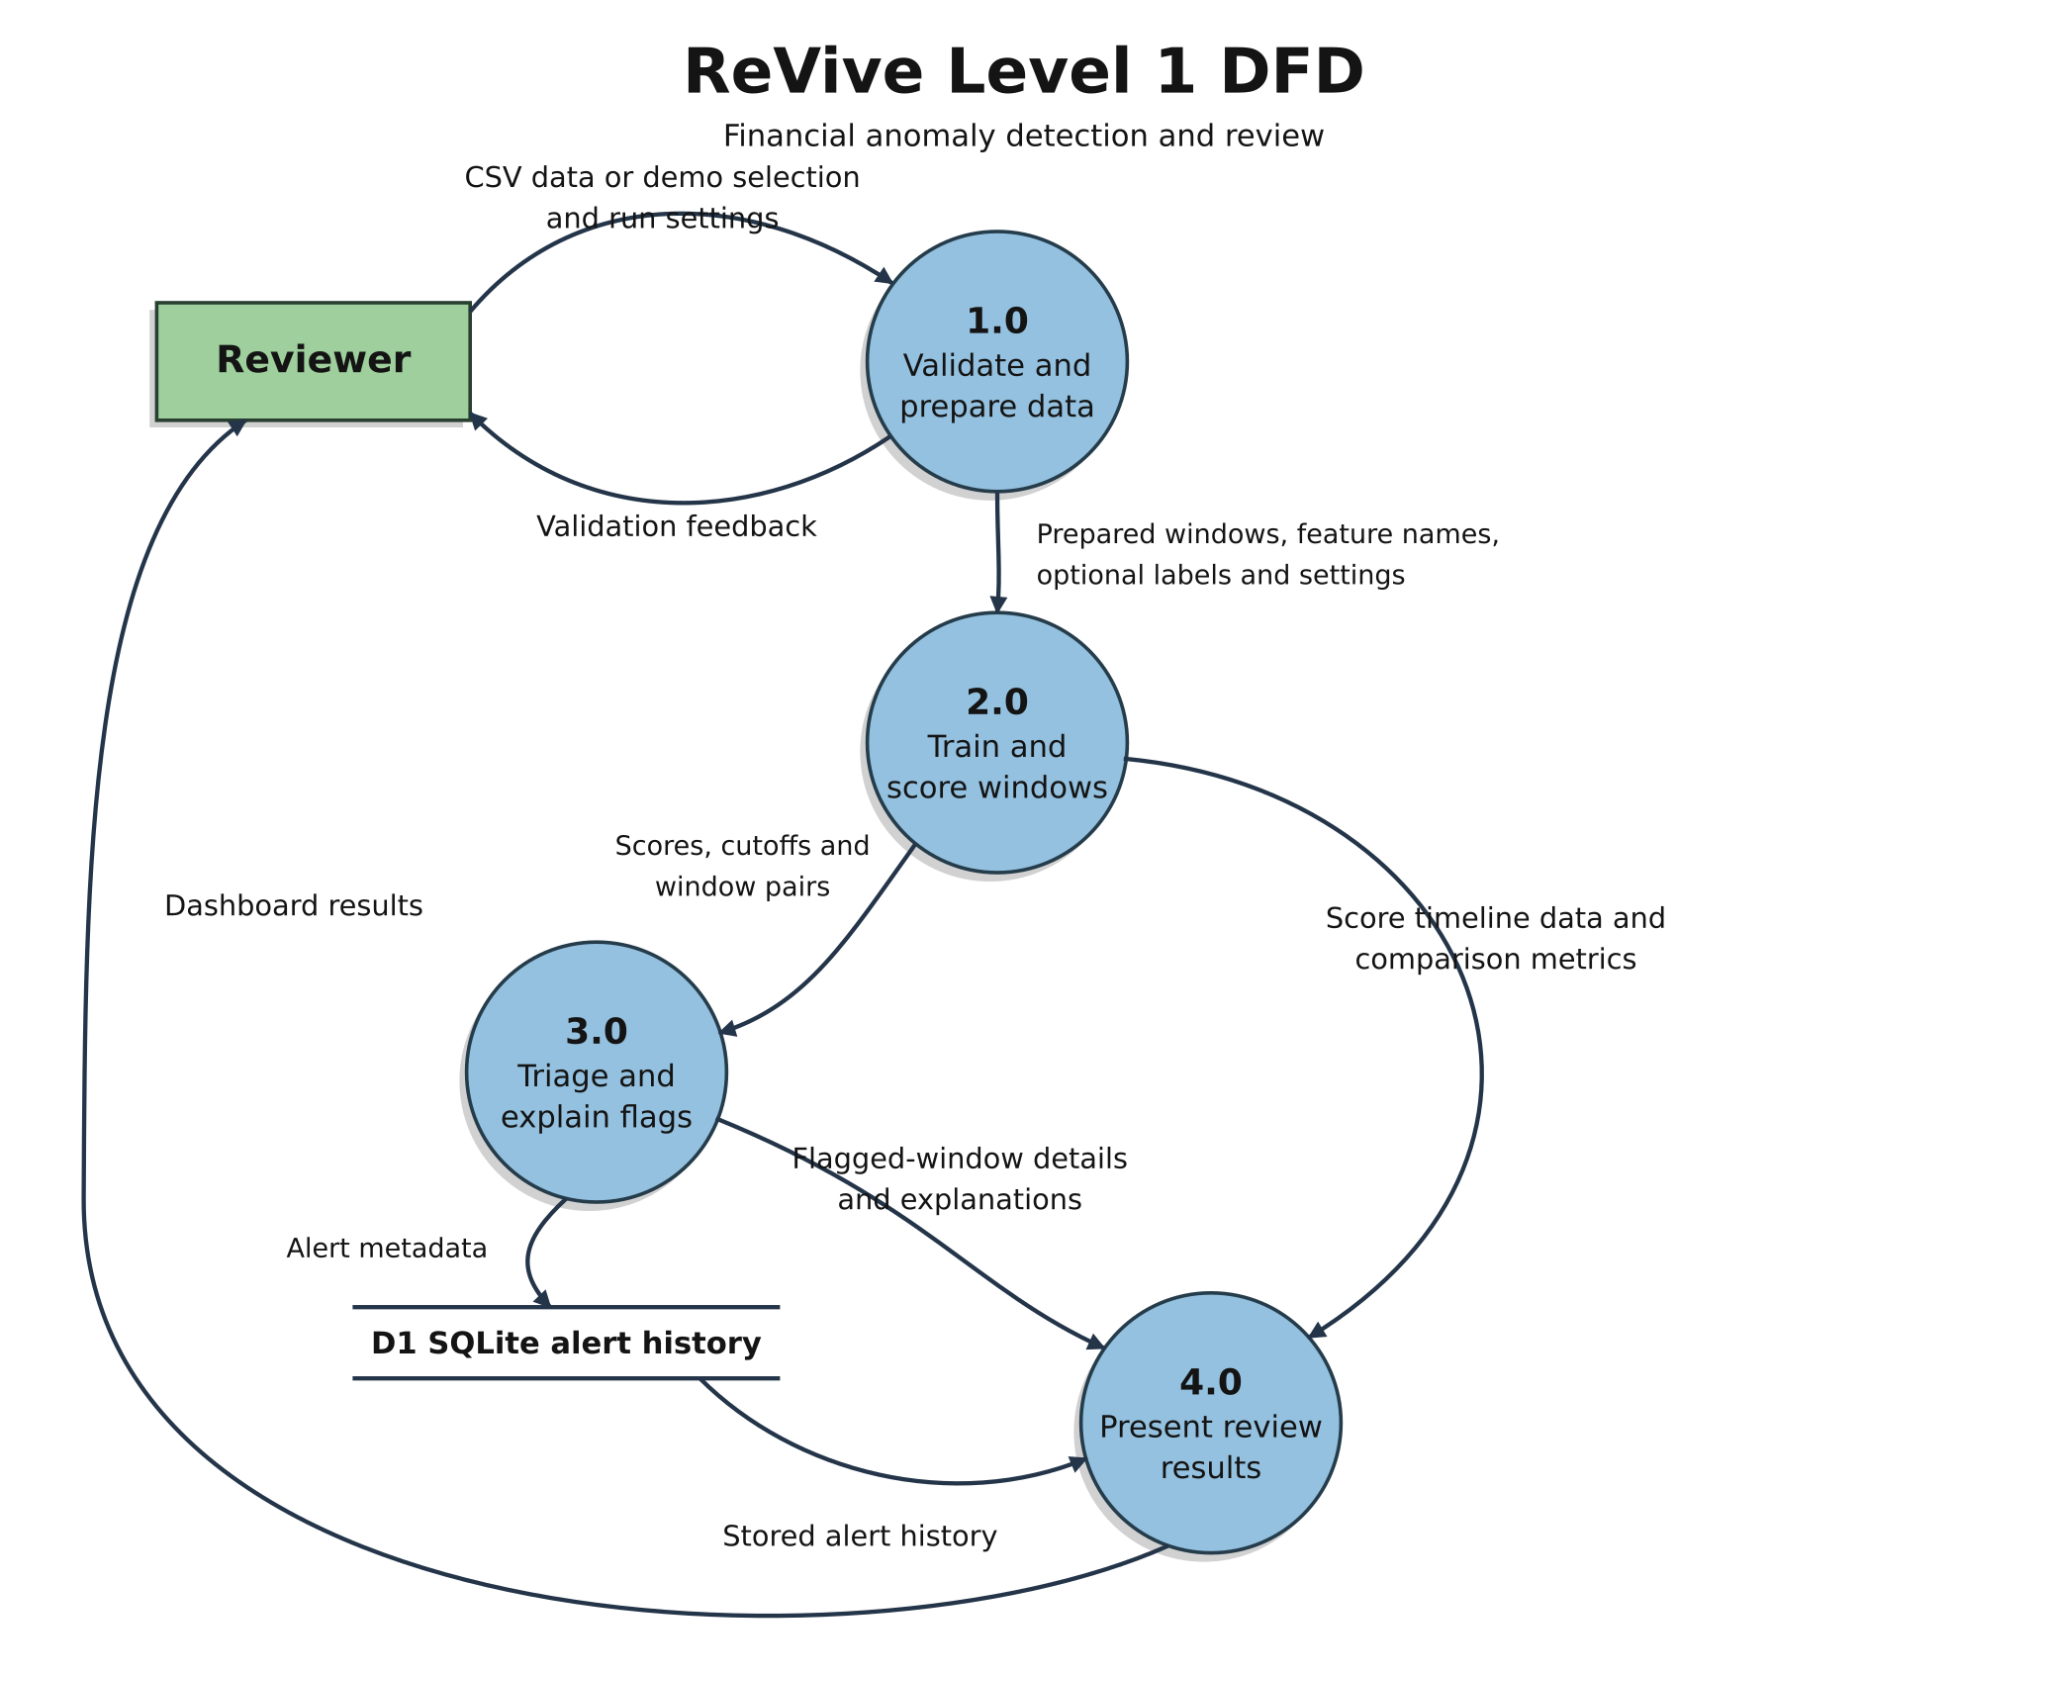
\includegraphics[width=\linewidth,height=4.65cm,keepaspectratio]{../docs/images/dfd-level-1.png}
\end{center}
\newpage
\heading{Sequence diagram}
\begin{center}
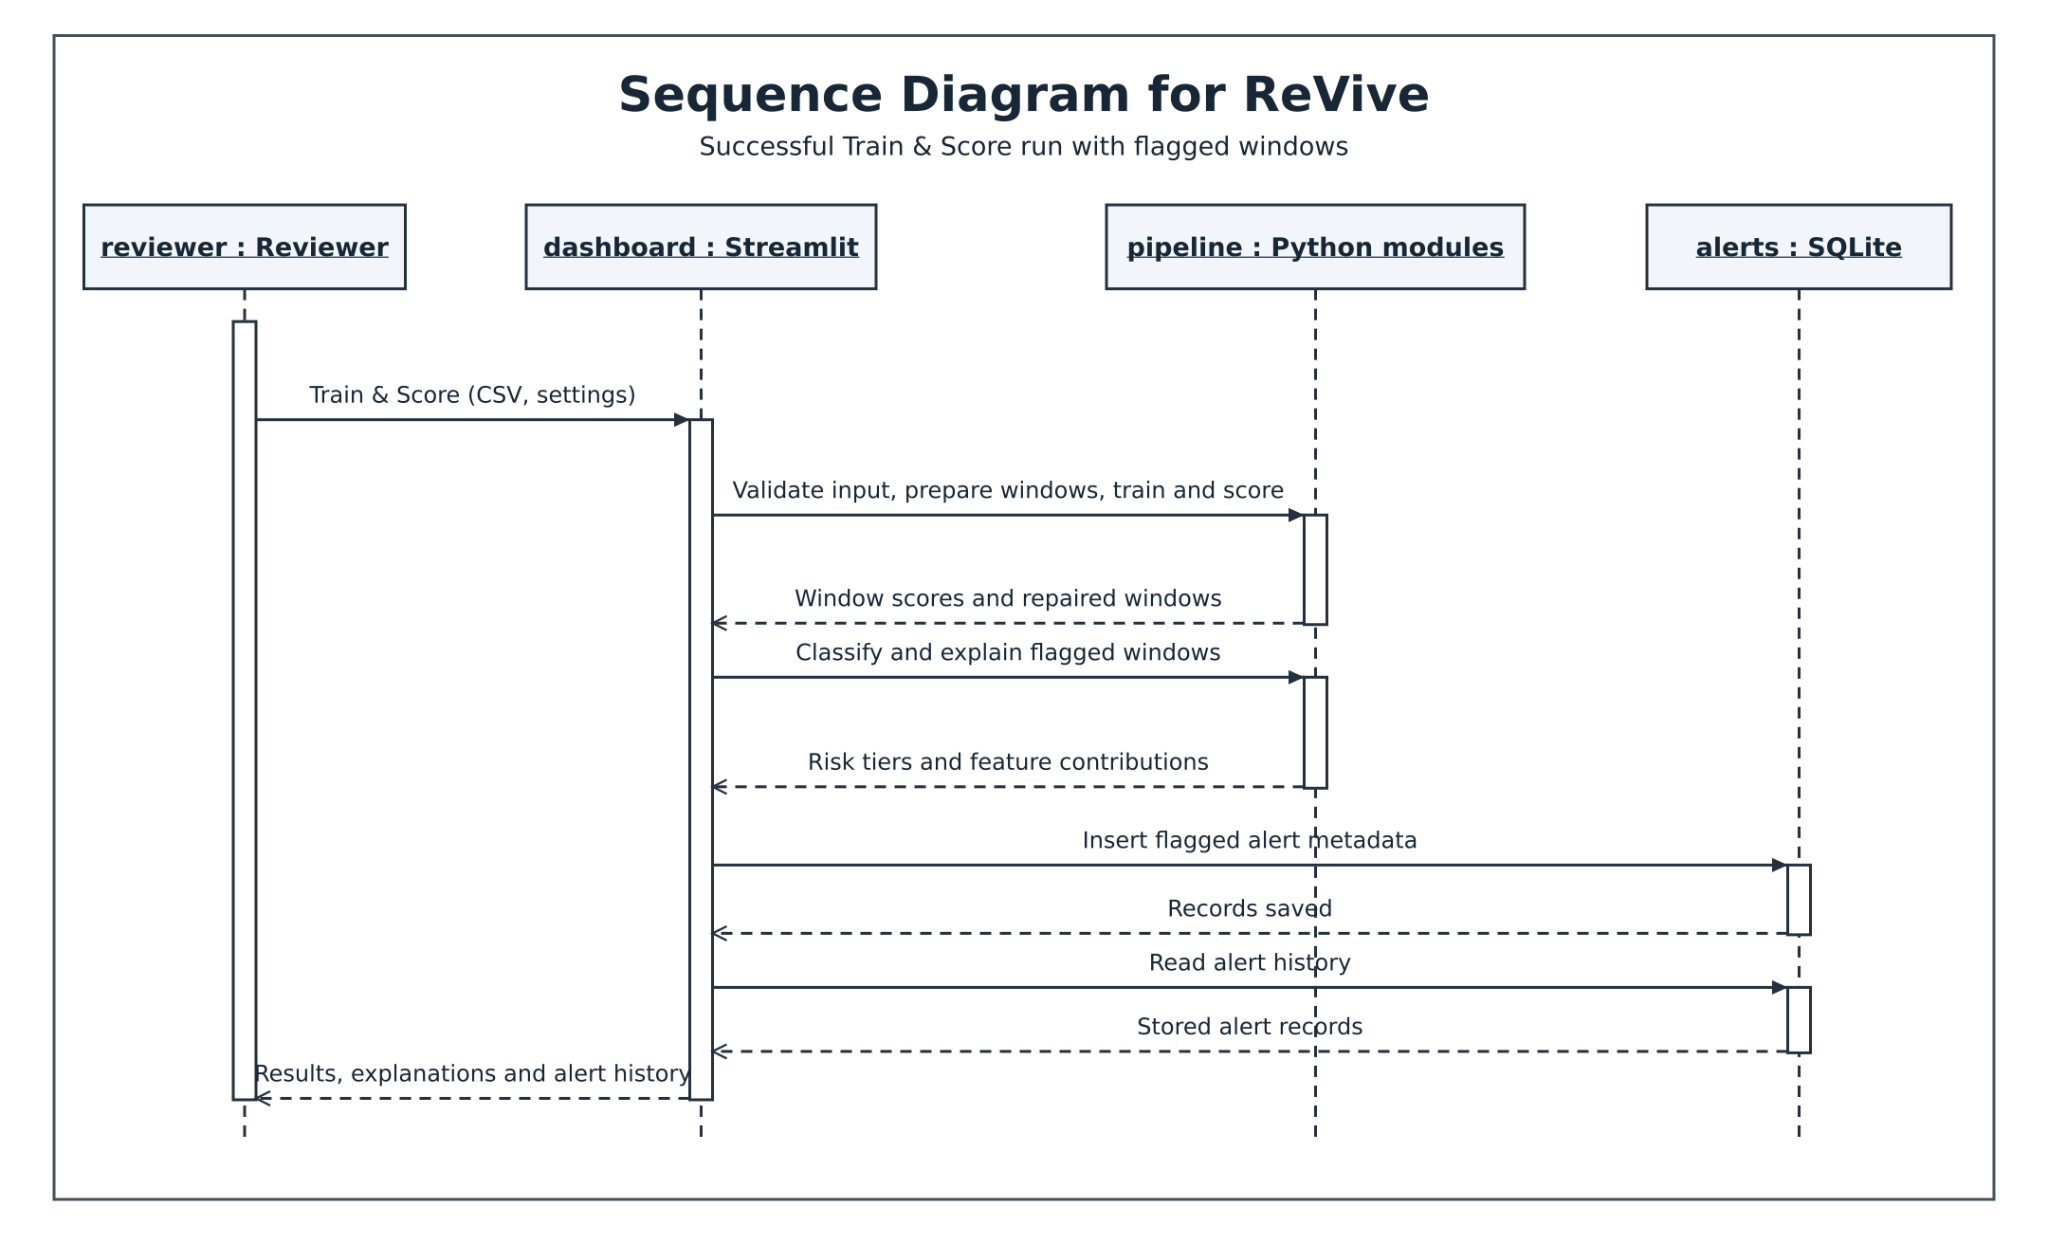
\includegraphics[width=\linewidth,height=4.65cm,keepaspectratio]{../docs/images/sequence-diagram.png}
\end{center}
\end{document}
